\section{Simulazione SITL}
\subsection{PID}
\subsubsection{STEP}
\todo[inline]{Tabella dei waypoints}
\begin{figure}
	\centering
	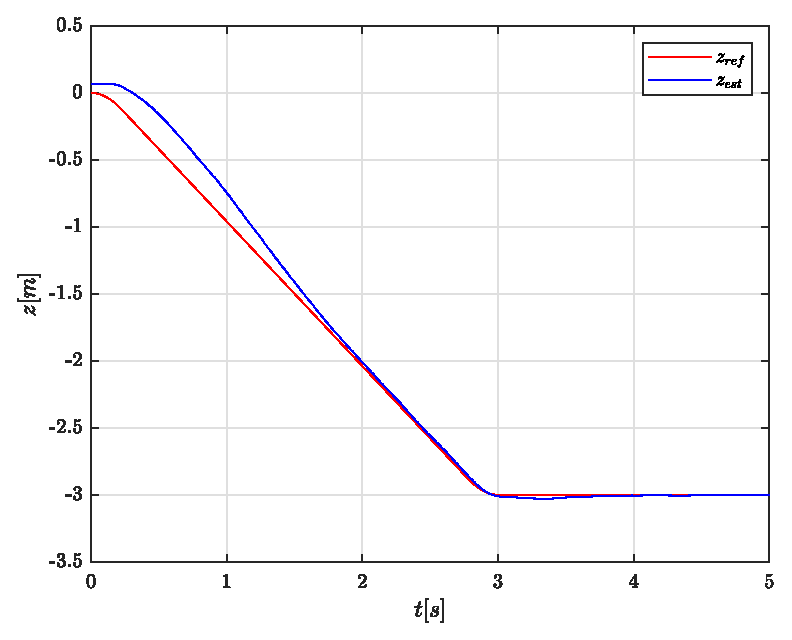
\includegraphics[width=0.5\textwidth]{Simulazioni/Figure/PID/STEP/AltitudeControlPos}
	\caption{Risposta con PID al segnale STEP : quota}
\end{figure}

\begin{figure}
	\centering
	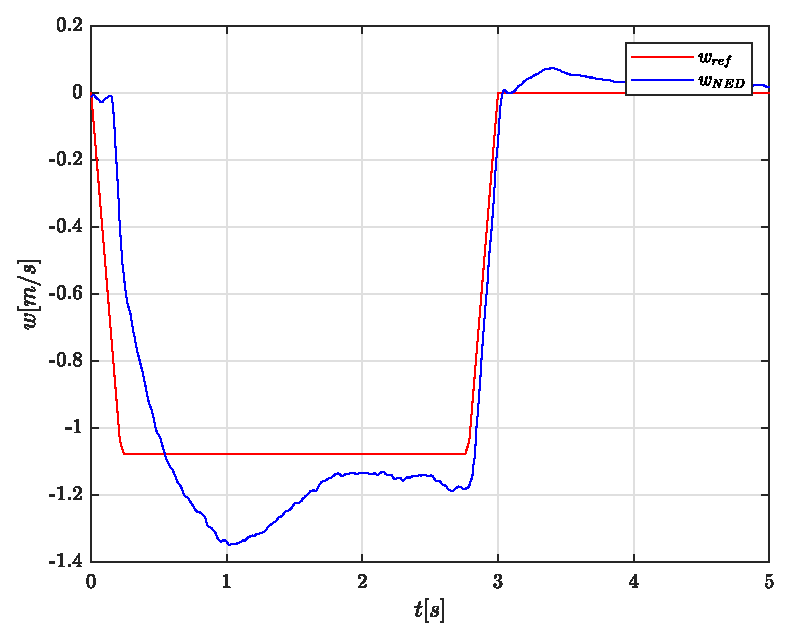
\includegraphics[width=0.5\textwidth]{Simulazioni/Figure/PID/STEP/AltitudeControlVel}
	\caption{Risposta con PID al segnale STEP : rateo di salita}
\end{figure}

\begin{figure}
	\centering
	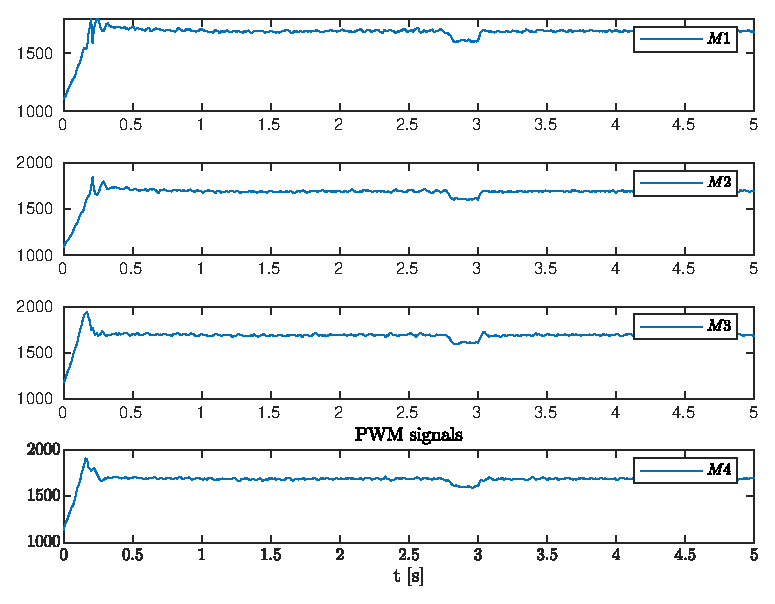
\includegraphics[width=0.5\textwidth]{Simulazioni/Figure/PID/STEP/PWM}
	\caption{Risposta con PID al segnale STEP : PWM}
\end{figure}

\clearpage
\subsection{SMC}
\subsubsection{STEP}
\todo[inline]{Tabella dei waypoints}
\begin{figure}
	\centering
	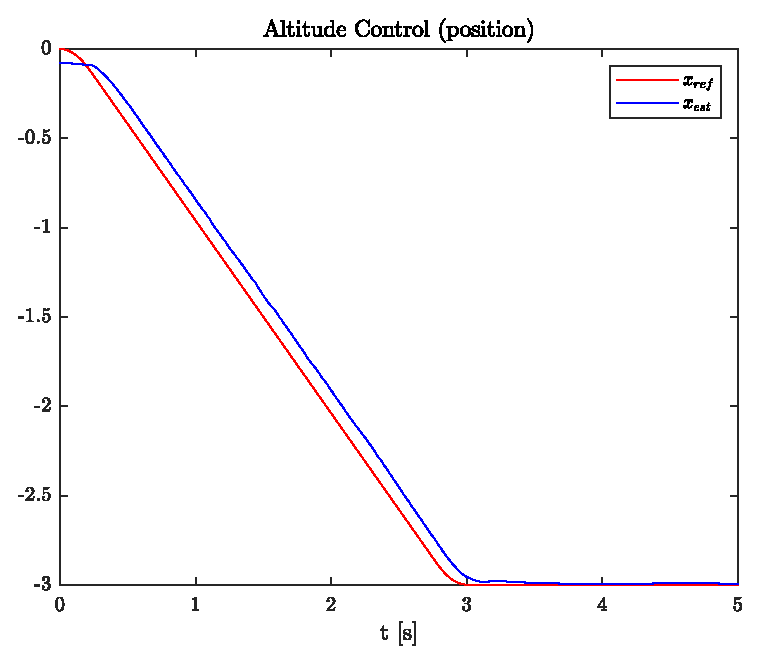
\includegraphics[width=0.5\textwidth]{Simulazioni/Figure/SMC/STEP/AltitudeControlPos}
	\caption{Risposta con PID al segnale STEP : quota}
\end{figure}

\begin{figure}
	\centering
	\includegraphics[width=0.5\textwidth]{Simulazioni/Figure/SMC/STEP/ALtitudeControlVel}
	\caption{Risposta con PID al segnale STEP : rateo di salita}
\end{figure}

\begin{figure}
	\centering
	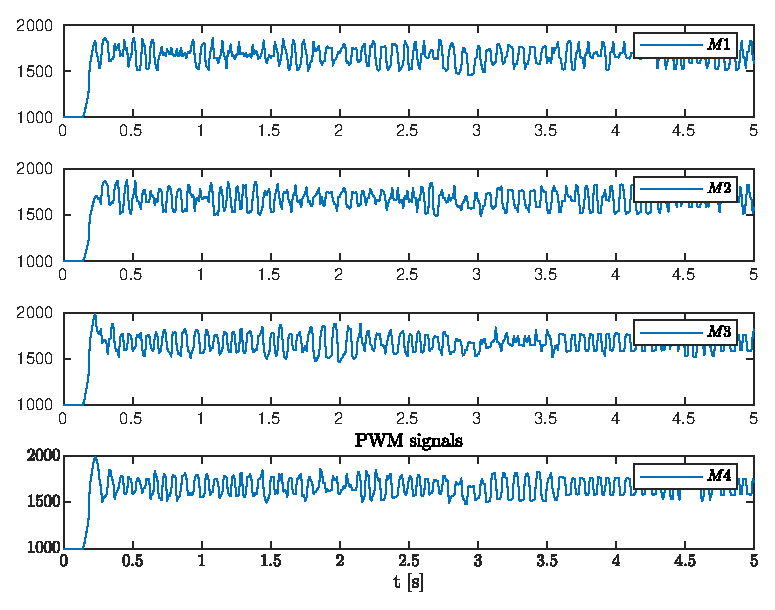
\includegraphics[width=0.5\textwidth]{Simulazioni/Figure/SMC/STEP/PWM}
	\caption{Risposta con PID al segnale STEP : PWM}
\end{figure}

\clearpage
\subsection{Confronto}